\documentclass[hyperref=unicode]{beamer}

\usepackage[absolute,overlay]{textpos}
\usepackage{graphicx}
\usepackage{adjustbox}
\usepackage{chemfig}
\usepackage[version=4]{mhchem}
\usepackage{wrapfig}
\usepackage{multirow}
\adjustboxset*{center}
\usepackage{caption}
\usepackage{chemformula}
\usepackage{elements}

%dělení slov
\usepackage{ragged2e}
\let\raggedright=\RaggedRight
%konec dělení slov

\usepackage{fontspec}
\usepackage{unicode-math}

\usepackage{polyglossia}
\setdefaultlanguage{czech}

\def\uv#1{„#1“}

\mode<presentation>{\usetheme{Madrid}}
\DefineNamedColor{named}{pozadi}{RGB}{200,200,200}
\usecolortheme{crane}

\setbeamertemplate{footline}[frame number]

\addtobeamertemplate{frametitle}{
	\let\insertframetitle\insertsectionhead}{}
\addtobeamertemplate{frametitle}{
	\let\insertframesubtitle\insertsubsectionhead}{}

\makeatletter
\CheckCommand*\beamer@checkframetitle{\@ifnextchar\bgroup\beamer@inlineframetitle{}}
\renewcommand*\beamer@checkframetitle{\global\let\beamer@frametitle\relax\@ifnextchar\bgroup\beamer@inlineframetitle{}}
\makeatother
\setbeamercolor{section in toc}{fg=blue}
\setbeamertemplate{section in toc shaded}[default][100]

\usepackage{tikz}
\usetikzlibrary{positioning}
\usetikzlibrary{arrows}
\usetikzlibrary{shapes.multipart}

\title[Crisis]
{Koordinační sloučeniny}

\subtitle{Koordinační sloučeniny, dativní vazba, ligandy, názvosloví, tvary komplexů, teorie ligandového pole}

\author{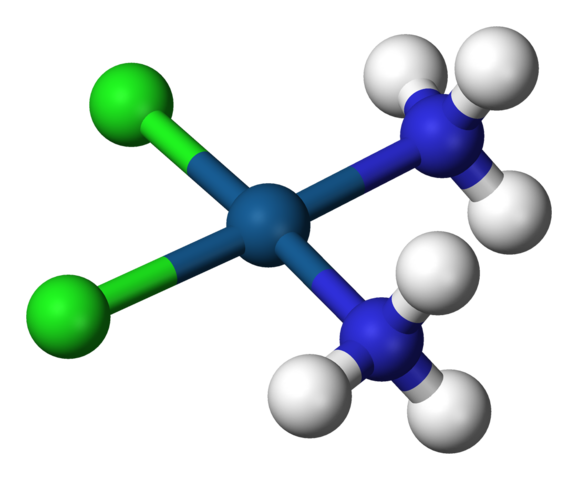
\includegraphics[keepaspectratio,width=4cm]{img/cisplatin.png}}
\date{}

\begin{document}
\frame{\titlepage}

\section{Koordinační sloučeniny}

\frame{
	\frametitle{}
	\begin{itemize}
	\item Koordinační sloučeniny jsou známy již dlouho, např. pruská modř.
	\item Jejich struktura byla ale dlouho neznámá, o její objasnění se zasloužil švédský chemik \emph{Alfred Werner}.
	\item Ve své struktuře obsahují alespoň jednu koordinační vazbu mezi centrálním kovem a ligandem.
	\item Koordinační vazba je dvouelektronová chemická vazba, kde oba elektrony pocházejí z jednoho atomu (\emph{donoru}), druhý atom (\emph{akceptor}) poskytuje pro tyto elektrony volný orbital.
	\item \ce{6 |NH3 + Co^{3+} -> [Co(NH3)6]^{3+}}
	\end{itemize}
}

\section{Ligandy}
\subsection{Hapticita, denticita}
\frame{
	\frametitle{}
	\begin{itemize}
	\item Ligandy jsou ionty nebo molekuly, které se váží na centrální atom. Nejčastěji vystupují jako Lewisovy báze, vzácněji i jako Lewisovy kyseliny.
	\item \emph{Denticita} - počet donorových atomů, kterými je ligand vázán k centrálnímu atomu.
	\begin{itemize}
	\item  \emph{Monodentátní ligandy} jsou vázány jedním atomem k centrálnímu kovu, např. \ce{NH3}
	\item  \emph{Bidentátní ligandy} jsou vázány dvěma atomy k centrálnímu kovu, např. ethylendiamin (en).
	\end{itemize}
	\end{itemize}
	\begin{center}
	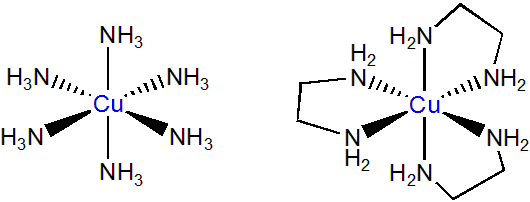
\includegraphics[keepaspectratio,width=7cm]{img/komplexy-chelaty.png}
	\end{center}
}

\subsection{Můstkové ligandy}
\frame{
	\frametitle{}
	\begin{itemize}
		\item Můstkové ligandy propojují dva nebo více centrálních kovů.
	\end{itemize}
	\begin{columns}
		\begin{column}{.5\textwidth}
			\begin{figure}
				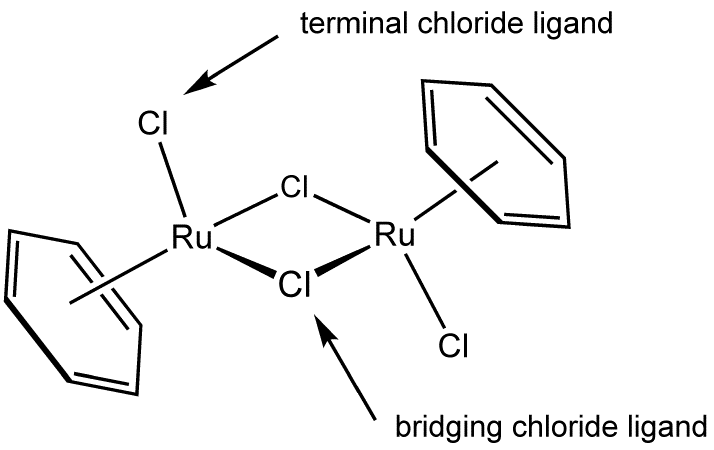
\includegraphics[height=.4\textheight]{img/Ru-Cl.png}
				\caption*{Ukázka komplexu s \ce{$\mu$_2-Cl} ligandem}
			\end{figure}
		\end{column}
		\begin{column}{.5\textwidth}
		\begin{figure}
			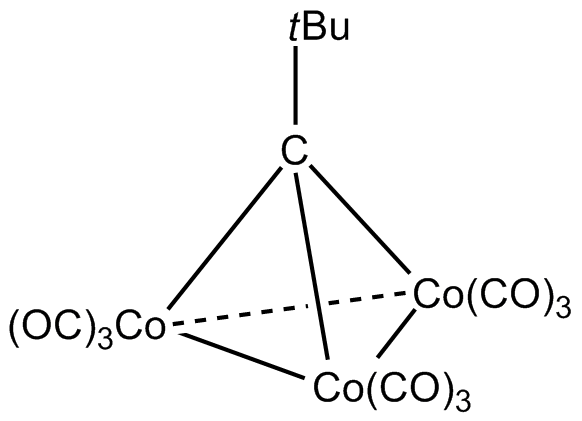
\includegraphics[height=.4\textheight]{img/Mu3_compound.png}
			\caption*{Ukázka komplexu s \ce{$\mu$_3-C^tBu} ligandem}
		\end{figure}
	\end{column}
	\end{columns}
}

\frame{
	\frametitle{}
	\begin{itemize}
	\item \emph{Hapticita} - vyjadřuje velikost (počet atomů) $\pi$-systému ligandu, kterým je vázán k centrálnímu atomu. Značí se řeckým písmenem eta ($\eta$).
	\item Ve ferrocenu je železnatý ion komplexován dvěma cyklopentadienylovými kruhy, vazba je vytvářena mezi železnatým iontem a celým $\pi$-systémem aniontu. Ligand pak označujeme jako $\eta^5$-cyklopentadienyl.
	\end{itemize}
	\begin{figure}
		\includegraphics[height=.4\textheight]{img/ferrocene.png}
	\end{figure}
}

\frame{
	\frametitle{}
	\textbf{Určení náboje centrálního atomu ze vzorce}
	\begin{itemize}
		\item V úvahu musíme vzít náboj iontu, protiontu i všech ligandů.
		\item \ce{[Co(NH3)6]Cl3}:
		\begin{itemize}
			\item Ve sloučenině jsou tři chloridové ionty, tzn. náboj komplexního iontu je 3+.
			\item Všechny ligandy mají nulový náboj.
			\item Kobalt musí mít tedy náboj 3+.
		\end{itemize}
		\item \ce{[Co(NH3)5Cl]Cl2}:
		\begin{itemize}
			\item Ve sloučenině jsou dva chloridové ionty, tzn. náboj komplexního iontu je 2+.
			\item Pět ligandů má nulový náboj, šestý ligand (\ce{Cl-}) nese jeden záporný náboj.
			\item Kobalt musí mít tedy náboj 3+.
		\end{itemize}
		\item \ce{[Pt(NH3)4][PtCl4]}
		\item \ce{K4[Fe(CN)6]}
		\item \ce{K3[Fe(CN)6]}
	\end{itemize}
}

\section{Názvosloví koordinačních sloučenin}
\frame{
	\frametitle{}
	Název těchto sloučenin se tvoří pojmenováním centrálního atomu a jednotlivých ligandů.
	\newline
	\newline

	\begin{tabular}{lll}
	\textbf{Vzorec} & \textbf{Ion} & \textbf{Ligand} \\
	\ce{SO$_4^{2-}$} & Síran & Sulfato- \\
	\ce{S2O$_3^{2-}$} & Thiosíran & Thiosulfato- \\
	\ce{PO$_4^{3-}$} & Fosforečnan & Fosfato- \\
	\ce{CH3COO^{-}} & Octan & Acetato- \\
	\ce{F^{-}} & Fluorid & Fluoro- \\
	\ce{Cl^{-}} & Chlorid & Chloro- \\
	\ce{O^{2-}} & Oxid & Oxido- \\
	\ce{H^{-}} & Hydrid & Hydrido- \\
	\ce{SCN^{-}} & Thiokyanatan & Thiokyanato- \\
	\end{tabular}
}

\subsection{Organické ligandy}
\frame{
	\frametitle{}

	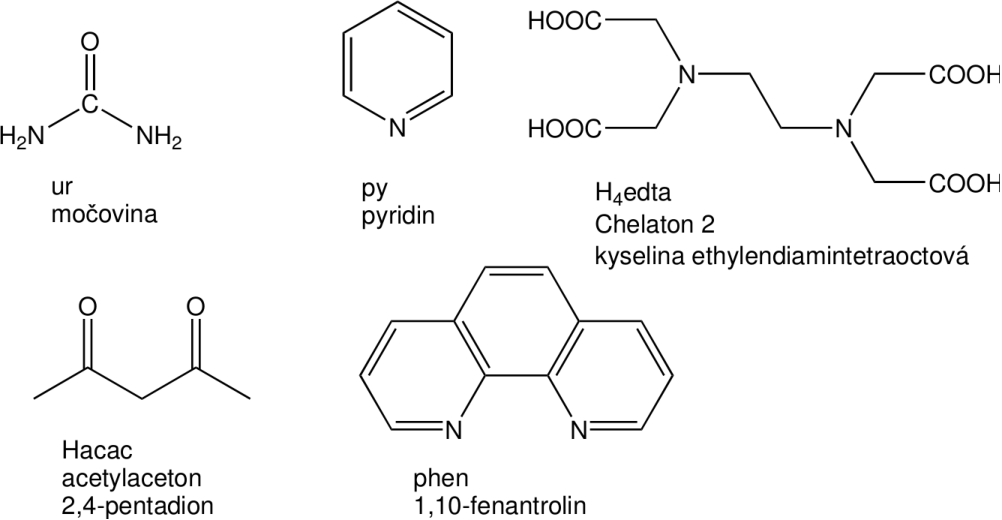
\includegraphics[keepaspectratio,width=105mm]{../01-nazvoslovi/ligandy.pdf}
}

\subsection{Izomerie}
\frame{
	\frametitle{}

	a) Ligand se koordinuje k centrálnímu atomu různými donorovými atomy. Jev se nazývá \textbf{vazebná izomerie} a izomery rozlišujeme rozdílnými názvy ligandů
\vspace{5mm}
\\
\begin{tabular}{llll}
\ce{-NO2} & nitro & \ce{-ONO} & nitrito \\
\ce{-SCN} & thiokyanato & \ce{-NCS} & isothiokyanato \\
\ce{-SeCN} & selenokyanato & \ce{-NCSe} & isoselenokyanato \\
\end{tabular}
\\
\vspace{10mm}
b) Koordinují se izomerní ligandy za vzniku \textbf{polohových izomerů}. I tento případ se vystihne rozdílným názvem ligandů
\vspace{5mm}
\\
\begin{tabular}{ll}
\textcolor{red}{H$_2$N}CH$_2$CH(\textcolor{red}{NH$_2$})CH$_3$ & 1,2-diaminopropan \\
CH$_3$\textcolor{red}{NH}CH$_2$CH$_2$\textcolor{red}{NH$_2$} & N-methylethylendiamin \\
\end{tabular}
}

\frame{
	\frametitle{}
c) Komplex má zaměněny ionty v koordinační a iontové sféře. Tuto situaci, nazývanou \textbf{ionizační izomerie}, řeší název komplexu
\\
\vspace{1cm}
\begin{tabular}{ll}
\ce{[Co(NH3)5SO4]Br} & bromid pentaammin-sulfatokobaltitý \\
\ce{[Co(NH3)5Br]SO4} & síran pentaammin-bromokobaltitý  \\
\end{tabular}
\vspace{1cm}
\\
d) U koordinačních sloučenin s komplexním kationtem i aniontem se může měnit rozdělení ligandů mezi koordinačními sférami obou centrálních atomů (\textbf{koordinační izomerie}) \\
\vspace{1cm}
\begin{tabular}{ll}
\ce{[Pt(NH3)4][CuCl4]} & tetrachloroměďnatan tetramminplatnatý \\
\ce{[Cu(NH3)4][PtCl4]} & tetrachloroplatnatan tetraamminměďnatý \\
\end{tabular}
}

\frame{
	\frametitle{}
	\begin{figure}
			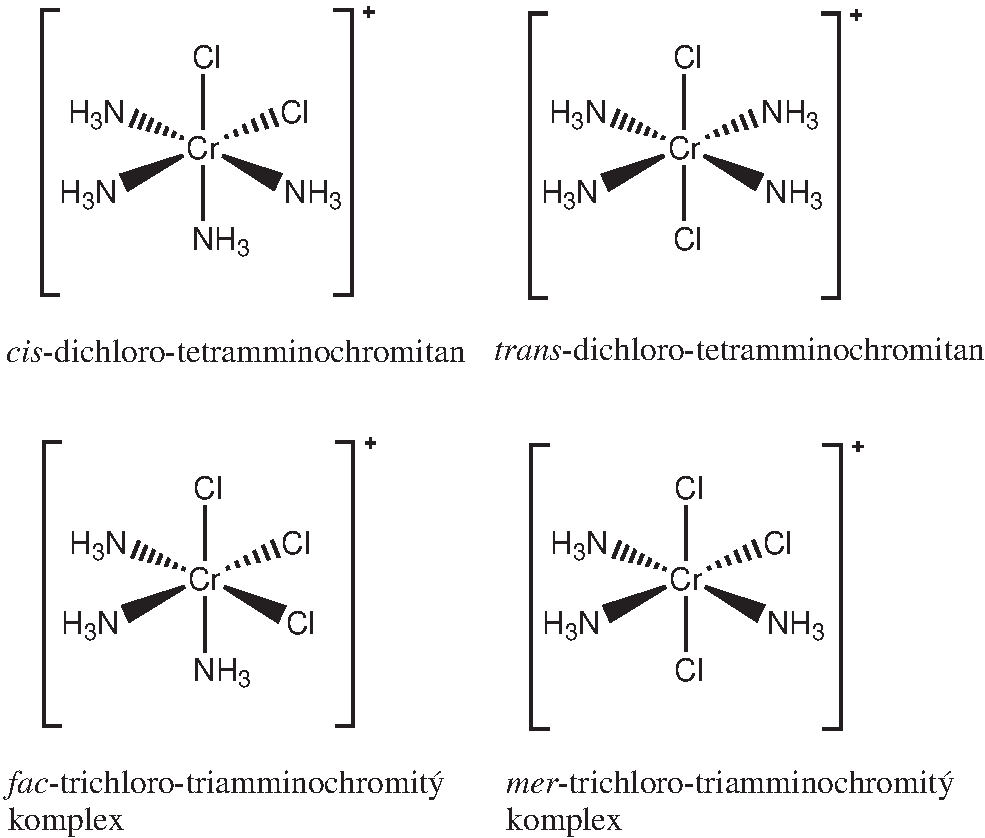
\includegraphics[height=.8\textheight]{../01-nazvoslovi/izomery.pdf}
	\end{figure}
}

\section{Teorie krystalového pole (CFT)}
\frame{
	\frametitle{}
	\begin{itemize}
	\item Popisuje vazebné poměry v koordinačních sloučeninách.
	\item Interakce mezi ligandem  a centrálním kovem je popisována pomocí elektrostatiky, ligandy jsou chápány jako negativní bodové náboje a kov jako kladný náboj.
	\item Vazba je realizována pomocí d-orbitalů kovu, které jsou v nevázaném iontu energeticky \emph{degenerované}, tzn. mají stejnou energii.
	\item Po vytvoření komplexu dojde, v závislosti na tvaru komplexu, k jejich rozštěpení na dvě skupiny. Velikost rozštěpení (rozdíl energií) je dána několika faktory:
	\begin{itemize}
	\item povahou a oxidačním stavem kovového iontu, čím je vyšší oxidační stav kovu, tím pozorujeme i silnější štěpení
	\item geometrickým uspořádáním ligandů okolo centrálního kovu
	\item povahou ligandu, čím silněji ovlivňuje ligand centrální kov, tím bude štěpení silnější
	\end{itemize}
	\item Sílu štěpení můžeme odhadnout pomocí spektrochemické řady ligandů, což je výčet ligandů seřazený podle síly generovaného pole:
	\begin{itemize}
	\item \ce{S^{2-}} < \ce{SCN^{–}} < \ce{Cl^{–}} < \ce{F^{–}} < \ce{OH^{–}} < \ce{H2O} < \ce{NH3} < \ce{CN^{–}} < \ce{CO}
	\end{itemize}
	\end{itemize}
}


\subsection{d-orbitaly}
\frame{
	\frametitle{}
	\begin{itemize}
	\item Existuje pět d-orbitalů, podle symetrie je můžeme rozdělit na dvě skupiny:
	\begin{itemize}
	\item \emph{t$_{2g}$} – sem patří tři orbitaly, jejichž laloky leží mezi osami souřadného systému, tj. $d_{xy}$, $d_{yz}$ a $d_{xz}$
	\item \emph{e$_g$} – dva orbitaly, jejichž laloky leží v osách souřadného systému, tj. $d_{z^2}$ a $d_{x^2-y^2}$.
	\end{itemize}
	\end{itemize}
	\begin{figure}
		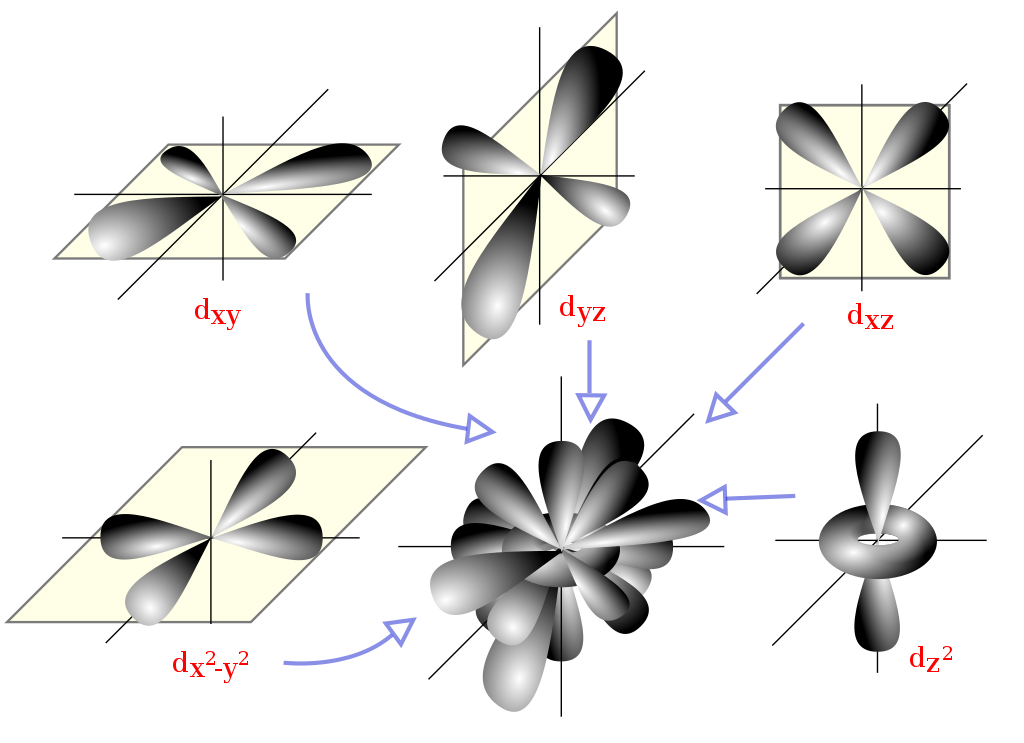
\includegraphics[height=.5\textheight]{img/D_orbitals.png}
	\end{figure}
}

\section{Teorie ligandového pole}
\frame{
	\frametitle{}
	\begin{itemize}
	\item Kombinace CFT a teorie molekulových orbitalů.\footnote[frame]{\href{https://chem.libretexts.org/Bookshelves/Inorganic_Chemistry/Supplemental_Modules_and_Websites_(Inorganic_Chemistry)/Ligand_Field_Theory/Ligand_Field_Theory_Fundamentals}{Ligand Field Theory Fundamentals}}
	\item Byla formulována roku 1957 Griffithem a Orgelem.\footnote[frame]{\href{http://pubs.rsc.org/en/content/articlelanding/1957/qr/qr9571100381}{Ligand Field Theory}}
	\item Teorie využívá elektrostatické interakce pro popis chování kovových iontů v roztoku a molekulových orbitalů pro popis rozdílů v interakcích mezi ligandy a kovem.
	\item Umožňuje odvodit barevnost a magnetické vlastnosti komplexů.
	\begin{itemize}
		\item \textit{Barevnost} je způsobena absorpcí části viditelného spektra. Během ní dochází k excitaci elektronu z t$_{2g}$ orbitalu do e$_{g}$.
		\item \textit{Magnetické vlastnosti} závisí na přítomnosti (\textit{paramagnetické komplexy}) nebo nepřítomnosti (\textit{diamagnetické komplexy}) nespárovaných elektronů.
	\end{itemize}
	\end{itemize}
}

\subsection{Multiplicita}
\frame{
	\frametitle{}
	\begin{itemize}
		\item Popisuje počet nepárových elektronů v komplexu.
		\item Je dána vztahem: M = 2S + 1, kde S je celkový spin komplexu.
	\end{itemize}

	\begin{tabular}{|l|l|l|l|}
	\hline
	\textbf{Počet nespárovaných elektronů} & \textbf{S} & \textbf{M} & \textbf{Označení} \\\hline
	0 & 0 & 1 & singlet \\\hline
	1 & $\frac{1}{2}$ & 2 & dublet \\\hline
	2 & 1 & 3 & triplet \\\hline
	3 & $\frac{3}{2}$ & 4 & kvartet \\\hline
	4 & 2 & 5 & kvintet \\\hline
	5 & $\frac{5}{2}$ & 6 & sextet \\\hline
	6 & 3 & 7 & septet \\\hline
	\end{tabular}
}

\subsection{Štěpení v oktaedrickém poli}
\frame{
	\frametitle{}
	\begin{itemize}
	\item Komplex se skládá z centrálního atomu a šesti ligandů, které jsou umístěny ve vrcholech oktaedru.
	\item Orbitaly $e_g$ si zvýší energii oproti neštěpeným d-orbitalům a orbitaly $t_{2g}$ si ji naopak sníží.
	\item Rozdíl mezi energetickými hladinami označujeme jako stabilizační energii oktaedrického pole ($\Delta_O$).
	\item V případě silných ligandů je hodnota $\Delta_O$ vyšší než hodnota párovací energie v d-orbitalech, proto se nejprve zcela zaplní orbitaly $t_{2g}$ a až poté se začnou plnit orbitaly $e_g$, vznikají tzv. \emph{nízkospinové komplexy}.
	\end{itemize}
	\begin{center}
	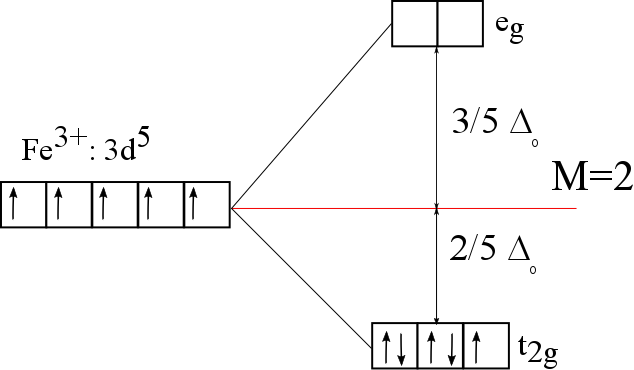
\includegraphics[keepaspectratio,width=40mm]{img/oktaedr-nizkospinovy.png}
	\end{center}
}

\frame{
	\frametitle{}
	\begin{center}
	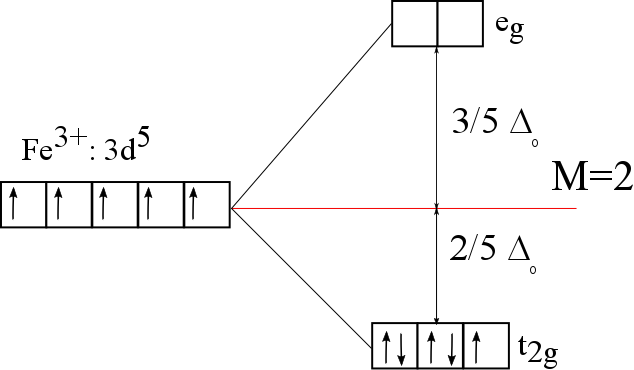
\includegraphics[keepaspectratio,width=110mm]{img/oktaedr-nizkospinovy.png}
	\end{center}
}

\frame{
	\frametitle{}
	\begin{itemize}
	\item V případě slabých ligandů je hodnota $\Delta_O$ nižší než hodnota párovací energie v d-orbitalech, pak je pro elektrony výhodnější nejprve zpola zaplnit všech pět orbitalů a až poté doplňovat elektronové páry v orbitalech. Vznikají tzv. \emph{vysokospinové komplexy}.
	\end{itemize}
	\begin{center}
	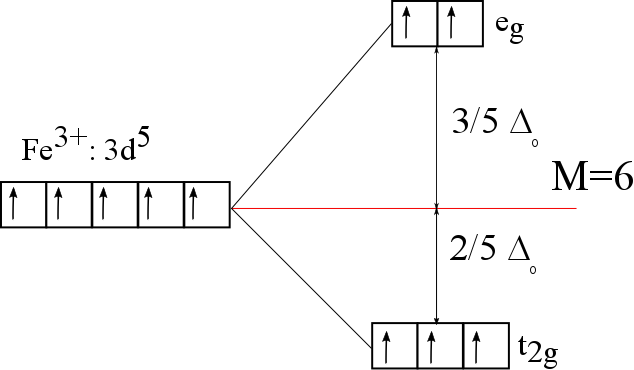
\includegraphics[keepaspectratio,width=80mm]{img/oktaedr-vysokospinovy.png}
	\end{center}
}

\subsection{Štěpení v tetraedrickém poli}
\frame{
	\frametitle{}
	\begin{itemize}
	\item Komplex se skládá z centrálního atomu a čtyř ligandů, které jsou umístěny ve vrcholech tetraedru.
	\item Štěpení orbitalů je opačné, $e_g$ jdou energeticky dolů a $t_{2g}$ nahoru.
	\item Síla tetraedrického pole ($\Delta_t$) je menší než polovina oktaedrického pole (přesně jde o $\frac{4}{9}\Delta_O$), proto jsou všechny tetraedrické komplexy vysokospinové.
	\end{itemize}
	\begin{center}
	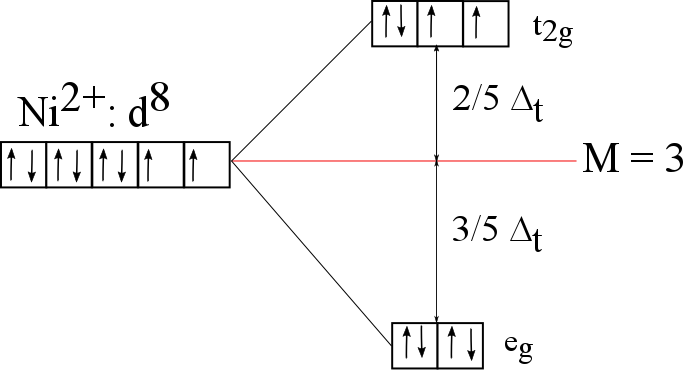
\includegraphics[keepaspectratio,width=80mm]{img/tetraedr-vysokospinovy.png}
	\end{center}
}

\section{Literatura}
\frame{
	\frametitle{}
	\setbeamertemplate{enumerate items}[default]
	\begin{enumerate}
	\item \href{http://doi.wiley.com/10.1002/hlca.19520350721}{Der Chelateffekt}
	\item \href{http://pubs.rsc.org/en/content/articlelanding/1957/qr/qr9571100381}{Ligand Field Theory}
	\item \href{https://chem.libretexts.org/Courses/University_of_California_Davis/UCD_Chem_002C/UCD_Chem_2C\%3A_Larsen/Text/Unit_2\%3A_Coordination_Chemistry/2.08\%3A_Bonding_in_Complex_Ions\%3A_Crystal_Field_Theory}{Bonding in Octahedral Complex Ions: Crystal Field Theory}
	\end{enumerate}
}

\iffalse
\section{Další informace}
\frame{
	\frametitle{}

	\href{http://z-moravec.net/chemie/zaklady-chemie/}{http://z-moravec.net/}
}
\fi

\end{document}